\CHAPTER{Introduction}
\label{chapter1}
\doublespace
\SECTION{Gravitational Waves}

Any theory of gravity that avoids instantaneous action at a distance
must feature some kind of gravitational waves.  Even Newtonian gravity
can be modified to account for propagation delays from massive bodies
that are the sources of attraction.  Gravity as we know it, however, is
described by the general theory of relativity. At the core of general
relativity is the Einstein field equation:

\begin{equation}
G_{\mu\nu} = \frac {8\pi G}{c^4} T_{\mu\nu}
\end{equation}

where $G_{\mu\nu} = R_{\mu\nu} - \frac{1}{2} R g_{\mu\nu}$ is the
Einstein tensor, $R_{\mu\nu}$ is the Ricci curvature tensor, $R$ is
the Ricci scalar, $g_{\mu\nu}$ is the spacetime metric, and $G$ is
(Newton's) universal gravitational constant.

\SECTION{Sources of Gravitational Waves}
Any system of mass accelerating in the quadrupolar or higher moments
will radiate energy into gravitational waves.  The effect is so weak,
however, that only some of the universe's more cataclysmic events have
a chance of producing waves observable on earth.

Anticipated sources of gravitational waves can be conveniently
catagorized as \emph{continuous} or \emph{transient}, and as
\emph{modeled} or \emph{unmodeled}.

\begin{itemize}
\item stochastic background
\item compact binary coalescence
\item pulsar (continuous wave)
\item bursts
\end{itemize}

Improvements in search sensitivity can be achieved by incorporating
knowledge of the expected signal waveform or spectrum; integrating
over a long period of time (for continuous sources); and by looking
for coincidence or coherence between multiple detectors.

The global network of gravitational wave detectors is operated as a
sensor array, an interferometer composed of many interferometers.

\SECTION{Detectors}
Gravitational waves couple to both light and matter.

\begin{figure}
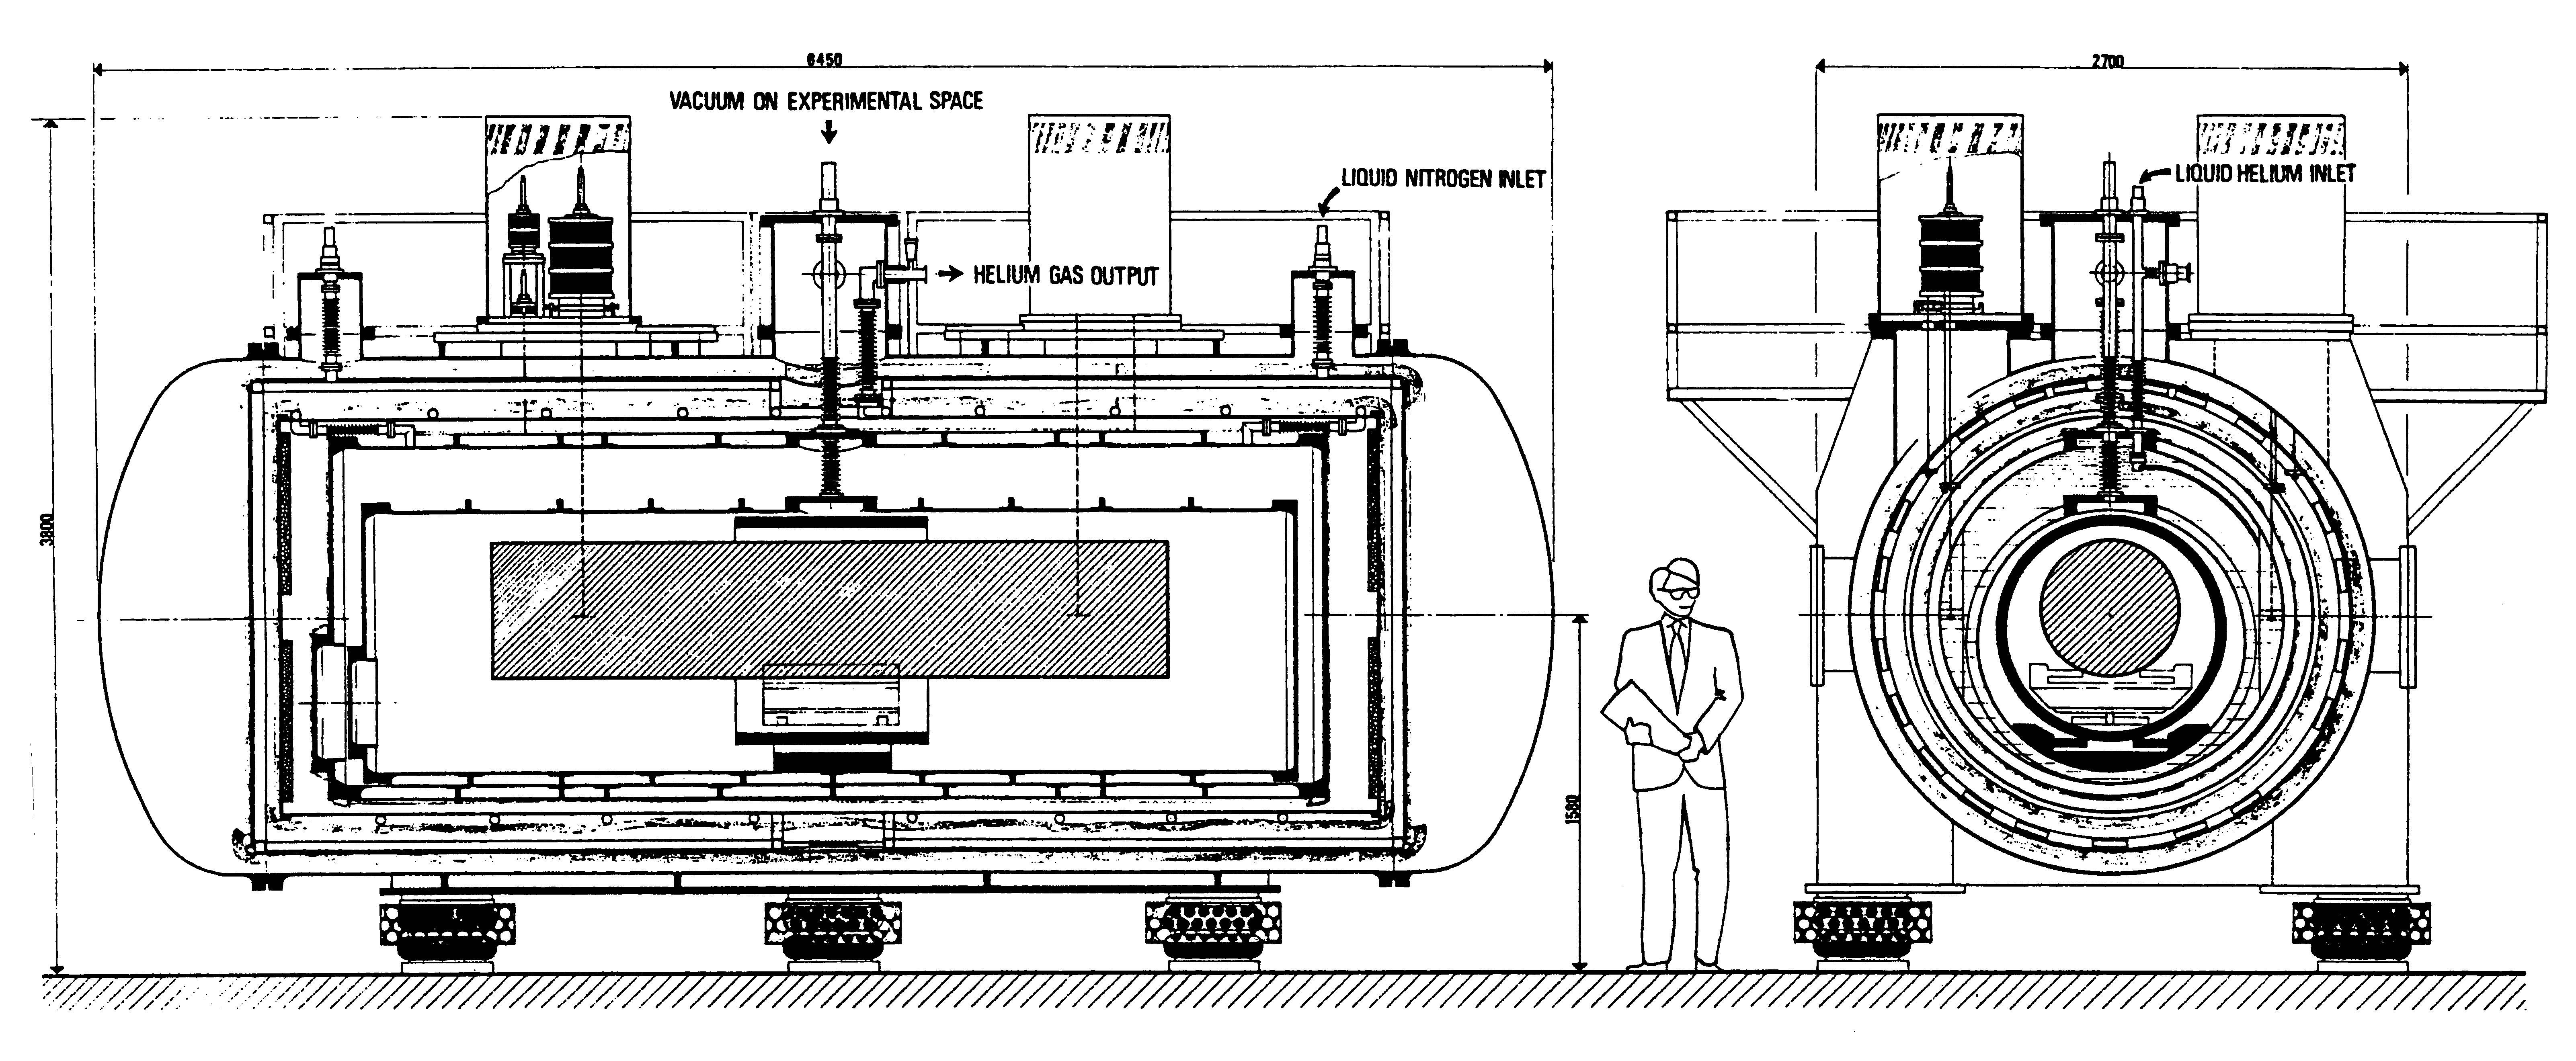
\includegraphics[width=\columnwidth]{chapter1/figures/explorer.png}
\caption{\label{fig:explorer-bar}Depiction of the cryostat of the EXPLORER bar detector, which operated \checkme{somewhere} for \checkme{some time}.  Illustration adapted from \checkme{a reference}.}
\end{figure}

The first attempts to detect gravitational waves used resonant bar
detectors.  In such a detector, a large chunk of a pure metal alloy
with a very high mechanical Q-factor is suspended in a vacuum chamber
and cooled to cryogenic temperatures.  A passing gravitational wave
couples mechanical energy into the bar, ringing up the fundamental
mechanical mode of the bar.  Sensitive detectors (latter bars used
SQUIDs) read out this mechanical displacement.  Resonant bars are
inherently narrow-band devices, sensitive to gravitational waves
within a narrow linewidth about their fundamental resonance.

Bar detectors do have the advantage that they are small enough to be
movable.

\SUBSECTION{Laser interferometers}
\cite{Weiss1972Electromagnetically,Forward1978Wideband}

Laser interferometers are now the instrument of choice in
the search for gravitational waves.  A gravitational wave will
modulate the optical path length of light traveling transversely
through it.  This path length modulation can be detected by a laser
interferometer.

A laser interferometer can, in principle, detect both polarization
components of the gravitational wave.  In practice, however, only one
polarization is sensed.

In terrestrial interferometers, inertial test masses are simulated by
hanging test masses as pendula.  The mass is free above the resonant
frequency of the pendulum, in the direction of the beam.

\SECTION{The Future}

It is hoped that Advanced LIGO, currently under construction, will
bring the first direct detection of gravitational waves and begin the
era of regular detection.

Several next-generation interferometers are in the works. 

The Einstein telescope is a planned system of three interferometers
with arms forming an equilateral triangle, to be installed in tunnels
deep under Europe.

Going into space makes feasible the use of extraordinarily long arms
and yields complete freedom from terrestrial noise, allowing access to
very low frequency gravitational waves.  The Laser Interferometer
Space Antenna design is composed of three spacecraft forming an
equilateral triangle, the whole constellation in solar orbit.  These
spacecraft will house truly inertial test-masses, floating within an
internal vacuum enclosure while external microthrusters keep the
spacecraft centered around the test mass.  The gravitational wave
channel is derived using time-delay interferometery.

\SECTION{This Dissertation}

This dissertation describes modifications to the initial LIGO
detectors that were undertaken between 2008 and 2010.  The state of
the LIGO detectors before these modifications is described in
\cite{S5InstrumentPaper} as well as numerous PhD dissertations,
notably Rana Adhikari's \cite{RanaThesis} and and Stefan Ballmer's
\cite{Ballmer2006LIGO}.

This dissertation does not address angular controls.
